\documentclass[[12pt,twoside]{book}
\usepackage{_my_document_style}
\begin{document}
%
\def\mySpanWingMT{16.000000}
\def\myMach{0.400000}
\def\myAspectRatioWing{9.142857}
\def\myChordRootWingMT{2.500000}
\def\myChordTipWingMT{1.000000}
\def\myTaperRatioWing{0.400000}
\def\myAreaWingMTsquared{28.000000}
\def\myCoeffAChordWing{-0.187500}
\def\myCoeffBChordWingMT{2.500000}
\def\myCLAlphaRootWingRAD{6.150000}
\def\myCLAlphaTipWingRAD{6.050000}
\def\myCoeffAClalphaWingRADMT{-0.012500}
\def\myCoeffAClalphaWingDEGMT{-0.000218}
\def\myCoeffBClalphaWingRAD{6.150000}
\def\myCLAlphaMeanWingRAD{6.107143}
\def\myCLAlphaMeanWingDEG{0.106590}
\def\myInducedDragFactorWing{0.902301}
\def\myCLAlphaWingRAD{4.942481}
\def\myCLAlphaWingDEG{0.086263}
\def\mySweepTmaxWingDEG{-0.540000}
\def\mySweepTmaxWingRAD{-0.009425}
\def\myDownwashGradientAtMachZeroHTail{0.330672}
\def\myDownwashGradientHTail{0.303066}
\def\mySweepQuarterChordWingRAD{0.000000}
\def\myXrWingMACQuarterChordToHTailMACQuarterChordMT{6.870000}
\def\myZrWingMACQuarterChordToHTailMACQuarterChordMT{0.320000}
\def\myFactorKARDownwashGradientHTail{0.087000}
\def\myFactorKmrDownwashGradientHTail{1.031000}
\def\myFactorKlambdaDownwashGradientHTail{1.257000}

%
\begin{myExampleX}{Gradient of the downwash angle (DATCOM method)}{\ding{46}}% \ \Keyboard\ %
\label{example:Wing:Downwash:B}
%
\noindent
Consider the same wing assigned
in the example~\ref{example:Wing:Downwash:A}.
We want to calculate the gradient \smash{$\diff{\epsilon}/\diff{\alpha}$} 
with a semiempirical formula which takes into account both the longitudinal position
of the horizontal tailplane and of its height with respect to the wing.

To estimate the gradient of $\diff{\epsilon}/\diff{\alpha}$ at the tail,
for subsonic flight regimes it can be used
the following analytical formula:
%\begin{equation}\label{eq:Aero:Fuselage:Aft:Downwash:Analytic}
\[
\frac{\diff{\epsilon}}{\diff{\alpha}} =
    \sqrt{1-M^2} \,
    \left[{%
    \num[round-precision=2]{4.44} \bigg( K_{\AR}\,K_{\lambda}\,K_\Htail
        \sqrt{\cos \Lambda_{c/4,\Wing}}\bigg)^{\num[round-precision=2]{1.19}}\,
    }\right]
\]
%\end{equation}
%valida anche per ali a freccia, 
with $\Lambda_{c/4}$ the sweep angle of the focus line. The multiplying factors
$K_{\AR}$, $K_{\lambda}$ and $K_\Htail$ take into account, respectively,
the aspect ratio $\AR$, the taper ratio $\lambda$ of the wing and the positioning of the horizontal tailplane.
They are expressed by the formulas
%\begin{equation}\label{eq:Aero:Fuselage:Aft:Downwash:KAR:Klam:KH}
\[
K_{\AR} = \frac{1}{\AR_\Wing}-\frac{1}{1+\AR_\Wing^{\num[round-precision=1]{1.7}}} \;,
\qquad
K_{\lambda} = \frac{10-3\,\lambda_\Wing}{7} \;,
\qquad
K_{\Htail} = \frac{1-\big(h_{\Htail\Wing}/b_\Wing\big)}{\;\;\,\big(2X_{\Htail\Wing}/b_\Wing\big)^{1/3}}
\]
%\end{equation}
where $h_{\Htail\Wing}$ is the vertical distance
of the aerodynamic center of the horizontal tail
from the mean aerodynamic chord of the wing
(or, for some authors, from the root chord $c_{\mathrm{r},\Wing}$ of the wing).
Conventionally $h_{\Htail\Wing}$ it is positive if the tail plane is located above the root chord.
The amount $X_{\Htail\Wing}$ is the longitudinal distance of the aerodynamic center
of horizontal tail
%dal punto a un quarto della corda di radice alare $c_{\mathrm{r},\Wing}$.
from the point to a quarter of the mean aerodynamic chord of the wing
(Or, for some authors point of view, from point a quarter of the root chord $c_{\mathrm{r},\Wing}$ of the wing).

In the example considered, we assume
\[
X_{\Htail\Wing} 
  = \SI[round-precision=2]{\myXrWingMACQuarterChordToHTailMACQuarterChordMT}{\meter}
  \;,\qquad
h_{\Htail\Wing}
  = \SI[round-precision=2]{\myZrWingMACQuarterChordToHTailMACQuarterChordMT}{\meter}
\]
where 
$\lambda_\Wing = \SI[round-precision=2]{\myTaperRatioWing}{}$ and
$b_\Wing = \SI[round-precision=0]{\mySpanWingMT}{\metre}$.
The point downstream of the wing where we want to evaluate the downwash gradient
is represented in the figure~\ref{fig:Wing:Downwash:B}.
We obtain
\[
K_{\AR} = \SI[round-precision=3]{\myFactorKARDownwashGradientHTail}{} \;,
\qquad
K_{\lambda} = \SI[round-precision=3]{\myFactorKlambdaDownwashGradientHTail}{} \;,
\qquad
K_{\Htail} = \SI[round-precision=3]{\myFactorKmrDownwashGradientHTail}{}
\]
\[
\left.\frac{ \diff{\epsilon} }{ \diff{\alpha} }\right|_{\Mach=0}
  = \left[{%
    \num[round-precision=2]{4.44} \,
    \bigg( 
      \SI[round-precision=3]{\myFactorKARDownwashGradientHTail}{}
      \cdot \SI[round-precision=3]{\myFactorKlambdaDownwashGradientHTail}{}
      \cdot \SI[round-precision=3]{\myFactorKmrDownwashGradientHTail}{}
        \sqrt{
          \cos \SI[round-precision=0]{ \mySweepQuarterChordWingRAD }{}
        }\bigg)^{\num[round-precision=2]{1.19}}\,
    }\right]
  = \mathunderline{mydarkblue}{ \SI[round-precision=2]{\myDownwashGradientAtMachZeroHTail}{} }
\]
and finally for a flight Mach number $\Mach=\SI[round-precision=2]{\myMach}{}$
\[
\frac{ \diff{\epsilon} }{ \diff{\alpha} }
  =
  \sqrt{1-\Mach^2} \,
  \left.\frac{ \diff{\epsilon} }{ \diff{\alpha} }\right|_{\Mach=0}
  = \sqrt{1-\SI[round-precision=2]{\myMach}{}^2} \,
    \cdot \SI[round-precision=2]{\myDownwashGradientAtMachZeroHTail}{}      
  = \mathunderline{mydarkblue}{ \SI[round-precision=2]{\myDownwashGradientHTail}{} }
\]
\end{myExampleX}
\begin{figure}
  [t]%[H]%[!htbp]
    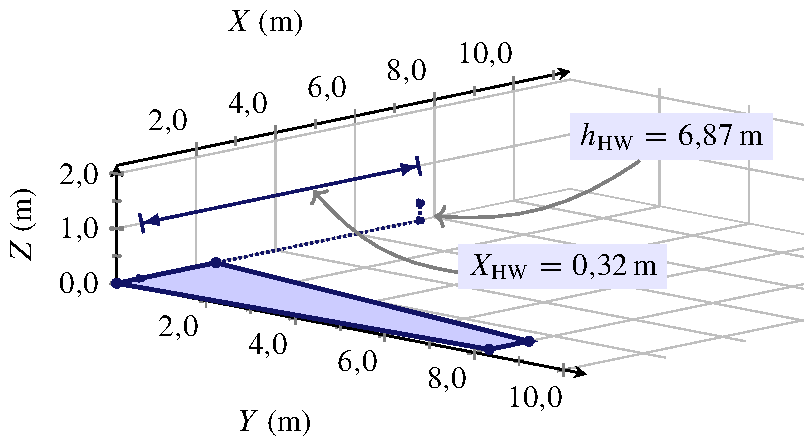
\includegraphics[width=0.70\textwidth]{Chapter_4/wing_downwash_2/wing_downwash_2_drawing.pdf}
  \caption{\finalhyphendemerits=1000
         Wing assigned in the example~\ref{example:Wing:Downwash:A}.
          The gradient $\diff{\epsilon}/\diff{\alpha}$ is calculated at a given point downstream of the wing.
  }
  \label{fig:Wing:Downwash:B}%
\end{figure}%
\end{document}